\documentclass[../bericht.tex]{subfiles}

\begin{document}

  \chapter{Versuchsdurchführung und -auswertung}

    Im folgenden Kapitel werden die einzelnen Schritte der Versuchsdurchführung und die jeweilige Analyse parallel beschrieben.


    \section{Vorbereitende Messungen}


      \subsection{Dunkelspektrum}

        Das Spektrometer zeichnet auch ohne Einschalten des Lasers bereits Signale auf. Dies liegt in diesem Falle nicht am Streulicht anderer Lichtquellen im Raum, wie durch das Ausbleiben von Veränderungen im Signal während dem Ein- und Ausschalten von prominenten Lichtquellen wie der Deckenleucchte leicht bewiesen werden kann. Vielmehr kommt es in der Ladungsträgerzone der Dioden zu spontanen Elektron-Loch-Paar-Bildungen, welche als Photonen registriert werden. Mit dem zu Auswertung verwendeten Programm \textit{???} wird deshalb bei jeder Änderung der Integrationszeit während der Versuche ein neues Dunkelspektrum aufgezeichnet, das heißt mit geblocktem Laserstrahl einmal die Integrationszeit durchlaufen. Dieses Dunkelspektrum subtrahiert das Programm dann von jedem weiteren aufgenommenen Spektrum automatisch, sodass der Untergrund weitgehen bereinigt ist.


      \subsection{Kalibrierung des Spektrometers}
      \label{subsec:kalibrierung}

        \begin{figure}[tb]
          \centering
          \tikzsetnextfilename{hg_he_spektren}
          \begin{tikzpicture}
            \begin{axis}[
              /tikz/line join=bevel,
              width=0.8*\textwidth,
              height=0.5*\textwidth,
              grid,
              legend style={at={(1,1)}, legend columns=1, anchor=north east},
              every axis plot,
              xmin = 490, xmax = 680,
              %ymin = \Pmin, ymax = \Pmax,
              xlabel = {Wellenlänge $\lambda$ in $\si{\nano\meter}$},
              ylabel = {Zählrate $n$},
              /pgf/number format/use comma,
              /pgf/number format/1000 sep={},
              ]
              % Add plots
              \addplot[color=red!30, only marks, line width = 1pt, mark options={scale=0.2}] table [x=lambda,y=n]{data/hg_spektrum_fit.txt};
              \addlegendentry{Hg data points}
              \addplot[color=red, line width = 1pt] table [x=lambda,y=fit]{data/hg_spektrum_fit.txt};
              \addlegendentry{Hg fit}
              \addplot[color=blue!30, only marks, line width = 1pt, mark options={scale=0.2}] table [x=lambda,y=n]{data/he_spektrum_fit.txt};
              \addlegendentry{He data points}
              \addplot[color=blue, line width = 1pt] table [x=lambda,y=fit]{data/he_spektrum_fit.txt};
              \addlegendentry{He fit}
            \end{axis}
          \end{tikzpicture}
          \caption{}
          \label{fig:hg-he-spektren}
        \end{figure}

        Um die Wellenlängen-, bzw. Frequenz-Kalibrierung des Spektrometers zu prüfen und gegebenenfalls zu korrigieren werden zwei Messungen mit in der Literatur hinreichend präzise charakterisierten Lichtquellen durchgeführt. Die aufgezeichneten Spektren einer Quecksilberdampflampe und einer Heliumlampe sind in \cref{fig:hg-he-spektren} abgebildet.  Die charakteristischen Linien treten hier verbreitert in Erscheinung. Es liegen die Dopplerverbreiterung, die Verbreiterung durch die natürliche Linienbreite, sowie die linear mit dem Dampfdruck ansteigende Druckverbreiterung vor. Prominent ist hierbei die Dopplerverbreiterung. Wegen der gaussförmigen Maxwell-Boltzmann-Verteilung der Geschwindigkeit der Gasatome können die verbreiterten Linien zu Bestimmung der Position der Maxima mit Gaussfits approximiert werden. Diese sind ebenfalls in \cref{fig:hg-he-spektren} aufgetragen. Die so gemessenen Linienpositionen mitsamt der aus \cite{NIST_ASD} entnommenen Literaturwerte sind in \cref{tbl:charakteristische-linien} aufgeführt. Die bei den experimentellen Werten angegebenen Unsicherheiten sind lediglich die Fehler der Fitparameter. Diese sind natürlich deutlich zu klein, wenn die Unsicherheiten aufgrund der  und Messunsicherheiten der verwendeten Geräte selbst noch respektiert werden. Dementsprechend stimmen die gemessenen Wellenlängen der charakteristischen Linien der Lichtquellen, vor Allem unter berücksichtigung der Breite der Guassglocken, hinreichend präzise mit den Literaturwerten überein, um keine weiteren Korrekturen vornehmen zu müssen.
        \medskip

        \begin{table}[tb]
        \caption[Experimentelle und Literaturwerte (\cite{NIST_ASD}) der charakteristischen Linien der Quecksilberdampflampe und der Heliumlampe.]{Experimentelle und Literaturwerte (\cite{NIST_ASD}) der charakteristischen Linien der Quecksilberdampflampe und der Heliumlampe zum Prüfen der Kalibrierung des Spektrometers. Für die weitere Interprätation siehe \cref{subsec:kalibrierung}}
        \label{tbl:charakteristische-linien}
        \selectfontsize{10pt}
        \begin{tabu} {X[r]X[r]X[r]X[r]X[r]X[r]X[r]}
          \unitoprule \\
          &\multicolumn3{c}{\textbf{Hg}}  &\multicolumn3{c}{\textbf{He}}  \\
          \unimidrule \\
          $\lambda_\mathrm{exp}$ $[\si{\nano\meter}]$ &546,075  &576,961  &579,067  &501,569  &587,562  &667.815 \\
          $\lambda_\mathrm{lit}$ $[\si{\nano\meter}]$ &546,237(1)  &577,128(2)  &579,241(3) &501,572(41)  &587,752(01)  &668,274(09) \\
          \unitoprule \\
        \end{tabu}
        \end{table}

        Natürlich ist der Nd:YAG-Laser. Ein Spektrum ohne Streuer wurde aber nicht aufgezeichnet und so soll hier vorab darauf verwiesen werden, dass das Maximum der Rayleigh-Streuung bezüglich der Raman-Verschiebung in allen späteren Messungen auf $\sim\SI{0}{\per\centi\meter}$ liegt und damit aufgrund der Einstellung des verwendeten Analyseprogramms bei $\SI{532}{\nano\meter}$. Dies bestätigt wiederum die zuvor gemachte Behaupttung, dass das Spektrometer hinreichend präzise für dieses Experiment kalibriert ist.


      \subsection{Linearität des Spektrometers}
      \label{subsec:linearitaet}

        \begin{figure}[tb]
          \tikzsetnextfilename{linearity}
          \begin{tikzpicture}
            \begin{axis}[
              /tikz/line join=bevel,
              width=0.8*\textwidth,
              height=0.5*\textwidth,
              grid,
              legend style={at={(1,1)}, legend columns=1, anchor=north east},
              every axis plot,
              xmin = 666, xmax = 671,
              %ymin = \Pmin, ymax = \Pmax,
              xlabel = {Wellenlänge $\lambda$ in $\si{\nano\meter}$},
              ylabel = {Zählrate $n$},
              ]
              % Add plots
              \addplot[color=red,  line width = 1pt] table [x=lambda,y=n]{data/he_50.txt};
              \addlegendentry{$\SI{50}{\milli\second}$}
              \addplot[color=blue,  line width = 1pt] table [x=lambda,y=n]{data/he_100.txt};
              \addlegendentry{$\SI{100}{\milli\second}$}
              \addplot[color=green,  line width = 1pt] table [x=lambda,y=n]{data/he_200.txt};
              \addlegendentry{$\SI{200}{\milli\second}$}
              \addplot[color=orange,  line width = 1pt] table [x=lambda,y=n]{data/he_400.txt};
              \addlegendentry{$\SI{400}{\milli\second}$}
              \addplot[color=purple,  line width = 1pt] table [x=lambda,y=n]{data/he_800.txt};
              \addlegendentry{$\SI{800}{\milli\second}$}
              \addplot[color=brown,  line width = 1pt] table [x=lambda,y=n]{data/he_2000.txt};
              \addlegendentry{$\SI{2000}{\milli\second}$}
              \addplot[color=violet,  line width = 1pt] table [x=lambda,y=n]{data/he_3000.txt};
              \addlegendentry{$\SI{3000}{\milli\second}$}
              \addplot[color=cyan,  line width = 1pt] table [x=lambda,y=n]{data/he_4000.txt};
              \addlegendentry{$\SI{4000}{\milli\second}$}
            \end{axis}
          \end{tikzpicture}
          \caption[Spektren der $\sim\SI{668}{\nano\meter}$-Linie der Heliumlampe bei verschiedenen Integrationszeiten zur Prüfung der Linearität des Spektrometers.]{Spektren der $\approx\SI{668}{\nano\meter}$-Linie der Heliumlampe bei verschiedenen Integrationszeiten zur Prüfung der Linearität des Spektrometers. Für weitere Ausführungen siehe \cref{subsec:linearitaet}}
          \label{fig:linearity}
        \end{figure}

        Das Spektrometer zählt unter Verwendung von Dioden die, nach Wellenlänge sortierten, einfallenden Photon. Bei zeitlich konstanter Lichtquelle sollte also die Zahl $n$ der registrierten Photonen pro wellenlänge linear zunehmen. Um dies zu überprüfen sind in \cref{fig:linearity} die Spektren der Heliumlampe für verschiedene Integrationszeiten aufgetragen. An dieser Stelle ist zu beachten, dass das Spektrometer 16 Bit basiert ist und damit eine Zählrate von $2^{16}\approx 65000$ nicht überschreiten kann.

        Die Zählrate der lokalen $\sim\SI{668}{\nano\meter}$-Maxima der Spektren werden mithilfe von \textit{Python} aus den Rohdaten extrahiert, deses Mal ohne die Verwendung eines Fits. Aufgetragen über den Integrationszeiten ergibt sich, wie erwartet, ein linearer Zusammenhang, wie in \cref{fig:linearitaet} abgebildet ist. Die Gleichung der linearen Regression durch den Ursprung ist
        \begin{equation}
          n(t_\mathrm{int})=\SI{8,386(1)}{\per\milli\second} \cdot t_\mathrm{int}.
          \label{eq:linear-fit}
        \end{equation}
        Messpunkte und Regression liegen übereinander, was die Linearität des Spektrometers unterhalb der Sättigungsgrenze bestätigt.

        \begin{figure}
          \tikzsetnextfilename{linear_fit}
          \begin{tikzpicture}
            \begin{axis}[
              /tikz/line join=bevel,
              width=0.8*\textwidth,
              height=0.5*\textwidth,
              grid,
              legend style={at={(1,0)}, legend columns=1, anchor=south east},
              every axis plot,
              xmin = 0, xmax = 5,
              ymin = 0, ymax = 35000,
              xlabel = {Integrationszeit $t_\mathrm{int}$ in $\si{\second}$},
              ylabel = {Zählrate $n$},
              /pgf/number format/use comma,
              /pgf/number format/1000 sep={},
              ]
              % Add plots
            	\addplot[color=red, only marks] coordinates {
            		(0.05,382.97)
            		(0.1,827.38)
            		(0.2,1605.61)
            		(0.4,3205.07)
            		(0.8,6782.87)
            		(2,16725.76)
            		(4,33572.35)
            	};
              \addlegendentry{Messpunkte}
              \addplot[color=blue, line width=1pt] gnuplot{8386.15286*x};
              \addlegendentry{Lineare Regression}
            \end{axis}
          \end{tikzpicture}
          \caption[Messpunkte der $\sim\SI{668}{\nano\meter}$-Maxima der Heliumlampen-Spektren bei verschiedenen Integrationszeiten (vgl. \cref{fig:linearity}) und lineare Regression.]{Messpunkte der $\sim\SI{668}{\nano\meter}$-Maxima der Heliumlampen-Spektren bei verschiedenen Integrationszeiten und lineare Regression gemäß \cref{eq:linear-fit}.}
          \label{fig:linearitaet}
        \end{figure}


      \subsection{Kerbfilter}
      \label{subsec:kerbfilter}

        Um die Breite und Position des Wellenlängenbereichs, welchen der Kerbfilter blockt, zu messen, wird eine Handytaschenlampe als breitbandige Lichtquelle genutzt. \Cref{fig:kerbfilter-spektren} zeigt Spektren des Handys mit und ohne Kerbfilte im Strahlengang. Dabei ist der Kerbfilter in der Nullposition $\varphi=0$ um $\ang{90}$ gegen den Strahlengang gedreht. Die weiteren Drehwinkel sind als Drehung gegen die Nullposition gemessen und aufgrund der Messung mittels Millimeterpapier stark Messunsicherheitsbehaftet ($\delta \varphi=\pm \ang{1}$). Durch die Drehung des Kerbfilters (Dünnschichtfilter) vergrößert sich die vom Licht zu transmittierende Schichtdicke und damit verschieben sich die geblockten Wellenlängen zu kleineren Werten. Hierbei ist die Verschiebung nach einfacher Geometrie unabhängig von der Drehrichtung. Die Breite des geblockten Wellenlängenintervalls wird in den folgenden Aalysen eine Rolle spielen.

        \begin{figure}[tb]
          \tikzsetnextfilename{kerbfilter}
          \begin{tikzpicture}
            \begin{axis}[
              /tikz/line join=bevel,
              width=0.8*\textwidth,
              height=0.5*\textwidth,
              grid,
              legend style={at={(1,1)}, legend columns=1, anchor=north east},
              every axis plot,
              xmin = 480, xmax = 660,
              %ymin = \Pmin, ymax = \Pmax,
              xlabel = {Wellenlänge $\lambda$ in $\si{\nano\meter}$},
              ylabel = {Zählrate $n$},
              /pgf/number format/use comma,
              /pgf/number format/1000 sep={},
              ]
              % Add plots
              \addplot[color=red,  line width = 1pt] table [x=lambda,y=n]{data/handy_ohne_kerb.txt};
              \addlegendentry{Ohne Kerbfilter}
              \addplot[color=blue,  line width = 0.5pt] table [x=lambda,y=n]{data/handy_mit_kerb.txt};
              \addlegendentry{$\varphi=\ang{0}$}
              \addplot[color=green,  line width = 0.5pt] table [x=lambda,y=n]{data/handy_mit_kerb_5_grad.txt};
              \addlegendentry{$\varphi=\ang{5}$}
              \addplot[color=orange,  line width = 0.5pt] table [x=lambda,y=n]{data/handy_mit_kerb_10_grad.txt};
              \addlegendentry{$\varphi=\ang{10}$}
              \addplot[color=magenta,  line width = 0.5pt] table [x=lambda,y=n]{data/handy_mit_kerb_15_grad.txt};
              \addlegendentry{$\varphi=\ang{15}$}
            \end{axis}
          \end{tikzpicture}
          \caption[Spektren einer Handytaschenlampe mit um den Winkel $\varphi$ gedrehten Winkel und ohne Kerbfilter.]{Spektren einer Handytaschenlampe mit um den Winkel $\varphi$ gedrehten Winkel und ohne Kerbfilter. Relevant ist die Verschiebung des durch den Kerbfilter entstehende Minimum des Transmissionsspektrum und dessen Verschiebung zu kürzeren Wellenlängen mit größer werdendem $\varphi$.}
          \label{fig:kerbfilter-spektren}
        \end{figure}


    \section{Probenanlayse}

      In diesem Abschnitt sollen die Spektren der gemessen Proben analysiert werden und damit Rückschlüsse auf die auftretenden Molekülschwingungen gezogen werden. Hierzu werden zunächst anhand eines einfachen harmonischen Oszillator Modells zweier Atome die zu erwartenden Raman-Verschiebungen in Abhängikeit der betiligten Elemente bestimmt (vgl. \cref{subsec:harm-oszi-absch}). Im Anschluss folgt die Betrachtung der aufgezeichneten Spektren und die Zuordnung derer Maxima zu Molekülschwinschungen.


      \subsection{Abschätzung der zu erwartenden Raman-Verschiebungen}
      \label{subsec:harm-oszi-absch}

        Als Basis der theoretischen Erwartung dient die Streckschwingung einer H-H-Bindung, deren Raman-Verschiebung nach \cite{herzberg} bei
        \begin{equation*}
          \nu_\mathrm{H-H}=\frac{1}{\lambda_0}-\frac{1}{\lambda}=\SI{4160}{\per\centi\meter},
        \end{equation*}
        mit der Wellenlänge des eingestrahlten Lichts $\lambda_0$ und der Wellenlänge der Raman-Maxima $\lambda$, liegt. Mit \cref{eq:omega} ergibt sich die Bindungsenergie des harmonischen Oszillators zu
        \begin{equation*}
          E=\frac{\mu}{2}\omega^2x_0^2=\frac{\mu}{2}\left[ 2\pi c \underbrace{\left( \frac{1}{\lambda_0} - \frac{1}{\lambda} \right)}_{=\nu} \right]^2x_0^2
        \end{equation*}
        wobei $\mu$ wie zuvor die reduzierte Masse ist und $c$ die Lichtgeschwindigkeit. Unter der Annahme, dass die Bindungsenergie für andere Atome gleich groß ist, folgt der Zusammenhang
        \begin{equation}
          \nu_\mathrm{Atom1-Atom2}=\sqrt{\frac{\mu_\mathrm{H-H}}{\mu_\mathrm{Atom-1-Atom2}}}\cdot \nu_\mathrm{H-H}.
          \label{eq:theo-raman-versch}
        \end{equation}
        Damit ergeben sich die in Tabelle \cref{tbl:theo-raman-versch} aufgeführten Raman-Verschiebungen für ausgewählte, in folgender Analyse relevanten, Atombindungen. Zur Berechnung wurden die in \cite{NIST_MASS} aufgeführten Atommassen verwendet.

        \begin{table}[tb]
        \caption[Theoretische Raman-Verschiebung verschiedener Atomkombinationen auf Grundlage des harmonischen Oszillator Modells unter Vorraussetzung der H-H-Bindungsenergie.]{Theoretische Raman-Verschiebung verschiedener Atomkombinationen auf Grundlage des harmonischen Oszillator Modells unter Vorraussetzung der H-H-Bindungsenergie. Die Werte wurden mit der Raman-Verschiebung einer H-H-Bindung $\nu_\mathrm{H-H}=\SI{4160}{\per\centi\meter}$ \cite{herzberg} und den in \cite{NIST_MASS} aufgeführten Atommassen nach \cref{eq:theo-raman-versch} berechnet.}
        \label{tbl:theo-raman-versch}
        \selectfontsize{10pt}
        \begin{tabu} {X[r]X[r]X[r]X[r]X[r]X[r]X[r]X[r]}
          \unitoprule \\
          &C-H  &C-D  &C-Cl &C-C  &O-H  &C-O  &N-O  \\
          \unimidrule \\
          $\Delta\nu$ $[\si{\nano\meter}]$ &3063 &2249 &988 &1206 &3033 &1128 &1081\\
          \unitoprule \\
        \end{tabu}
        \end{table}


      \subsection{Tetrachlormethan}
      \label{subsec:tetrachlor}

        \begin{figure}[tb]
          \tikzsetnextfilename{CCl4}
          \begin{tikzpicture}
            \begin{axis}[
              /tikz/line join=bevel,
              width=0.8*\textwidth,
              height=0.5*\textwidth,
              grid,
              legend style={at={(1,1)}, legend columns=1, anchor=north east},
              every axis plot,
              xmin = -1000, xmax = 1000,
              %ymin = \Pmin, ymax = \Pmax,
              xlabel = {Raman-Verschiebung $\Delta \nu$ in $\si{\per\centi\meter}$},
              ylabel = {Zählrate $n$},
              /pgf/number format/use comma,
              /pgf/number format/1000 sep={},
              ]
              % Add plots
              \addplot[color=red,  line width = 1pt] table [x=raman,y=n]{data/CCl4_pol0.txt};
              \addlegendentry{$\theta_\mathrm{pol}=\ang{0}$}
            \end{axis}
          \end{tikzpicture}
          \caption[Spektrum der $\mathrm{CCl_4}$-Probe mit Polarisationsfilter in der Nullstellung.]{Spektrum der $\mathrm{CCl_4}$-Probe mit Polarisationsfilter in der Nullstellung. Die Raman Linien treten klar als Maxima hervor, welche symmetrisch nach links, bzw. rechts relativ zum Rayleigh-Maximum ($\Delta \nu = \SI{0}{\per\centi\meter}$) verschoben sind. Das Nichterscheinen einiger Maxima auf negativer Seite geht auf die Unterdrückung durch den Kerbfilter zurück.}
          \label{fig:ccl4}
        \end{figure}

        \Cref{fig:ccl4} zeigt das Spektrum der Tetrachlormethan-Probe ($\mathrm{CCl_4}$) mit eingesetztem Polarisationsfilter. Der Winkel $\theta_\mathrm{pol}$ gibt hierbei den Drehwinkel des Polarisationsfilter an, wobei $\theta=\ang{0}$ die Nullpolarisationsstellung bezeichnet. Bei letzter Einstellung sind alle Raman-Maxima sichtbar, symmetrische und nicht-symmetrische. Weiter liegt der Kerbfilter im Strahlengang, um das prominente Maximum der Rayleigh-Streuung zu schwächen. Da der Wellenlängenbereich, welcher durch den Kerbfilter unterdrückt wird, recht breit ist (vgl. \cref{subsec:kerbfilter}), verschwinden hierdurch auch die einige der Raman-Maxima auf der linken Seite (negative Raman-Verschiebung) des Rayleigh-Maximums. Da die Stokes- und Anti-Stokes-Maxima aber symmetrisch um das Rayleigh-Maximum verteilt liegen, reicht es für die Charakterisierung der Raman-Linien eine Seite zu betrachten.
        \medskip

        \begin{figure}[tb]
          \tikzsetnextfilename{CCl4_beide}
          \begin{tikzpicture}
            \begin{axis}[
              /tikz/line join=bevel,
              width=0.8*\textwidth,
              height=0.5*\textwidth,
              grid,
              legend style={at={(1,1)}, legend columns=1, anchor=north east},
              every axis plot,
              xmin = 0, xmax = 1600,
              %ymin = \Pmin, ymax = \Pmax,
              xlabel = {Raman-Verschiebung $\Delta \nu$ in $\si{\per\centi\meter}$},
              ylabel = {Zählrate $n$},
              /pgf/number format/use comma,
              /pgf/number format/1000 sep={},
              ]
              % Add plots
              \addplot[color=red,  line width = 1pt] table [x=raman,y=n]{data/CCl4_pol0.txt};
              \addlegendentry{$\theta_\mathrm{pol}=\ang{0}$}
              \addplot[color=blue,  line width = 1pt] table [x=raman,y=n]{data/CCl4_pol1.txt};
              \addlegendentry{$\theta_\mathrm{pol}=\ang{90}$}
            \end{axis}
          \end{tikzpicture}
          \caption[Spektren der $\mathrm{CCl_4}$-Probe mit Polarisationsfilter in Nullstellung $\theta=\ang{0}$ und im Drehwinkel $\theta=\ang{90}$.]{Spektren der $\mathrm{CCl_4}$-Probe mit Polarisationsfilter in Nullstellung $\theta=\ang{0}$ und im Drehwinkel $\theta=\ang{90}$. Aufgrund der Symmetrie von Stokes- und Anti-Stokes-Maxima ist nur die positive Seite des Spektrums dargestellt. Das Verschwinden des $\sim\SI{451}{\per\centi\meter}$-Maximums bei gedrehtem Polarisationsfilter zeigt, dass die zugehörige Schwingung symmetrisch ist (und die anderen, nichtverschwindenden nicht symmetrisch).}
          \label{fig:ccl4-beide-pol}
        \end{figure}

        \Cref{fig:ccl4-beide-pol} zeigt nun den positiven Bereich der Raman-Verschiebung der $\mathrm{CCl_4}$-Probe mit Polarisationsfilter in der Nullstellung und der um $\ang{90}$ gedrehten Stellung. Insgesamt sind für die Nullpolarisationsstellung sechs oder sieben Raman-Maxima zu erkennen. An dieser Stelle ist noch unklar, ob das Maximum des Signals bei $\sim \SI{777}{\per\centi\meter}$ zu einem einzelnen Singulett oder zwei dicht beieinanderliegenden Linien eines Dupletts gehört.

        Nun lässt sich aufgrund der in \cref{subsec:harm-oszi-absch} berechneten theoretischen Raman-Verschiebung von $\SI{988}{\per\centi\meter}$ für eine einfache C-Cl-Bindung das Maximum bei $\sim \SI{1533}{\per\centi\meter}$ als Fundamentalschwingung ausschließen. Damit verbleiben noch vier oder fünf Maxima.

        Bei Betrachtung des Spektrum mit $\theta=\ang{90}$ fällt auf, dass nur die zum Maximum bei $\sim\SI{451}{\per\centi\meter}$ gehörende Schwingung polarisiert ist, während alle anderen depolarisiert sind.

        \Cref{fig:tetraeder-schwingungen} zeigt die möglichen Schwingungen eines $\mathrm{XY_4}$-Moleküls (X, Y seien Elemente). Offensichtlich sind drei Schwingungen in der zweiten, bzw. dritte Zeile mit Drehungen und Spiegelungen an Ebenen ineinander überführbar. Das heißt die Schwingungen sind dreifach entartet und es sind insgesamt vier Fundamentalschwingungen zu erwarten. Die einzige symmetrische Schwingung ist die Schwingung $\nu_1$, welche somit dem Maximum bei $\sim\SI{451}{\per\centi\meter}$ zugeordnet werden kann.
        \medskip

        Weiter lässt sich die Streckschwingung eines C-Cl-Paares als Superposition der $\nu_{3i}$, $i\in\{ a,b,c\}$ darstellen. Für die Streckschwingung wurde in \cref{subsec:harm-oszi-absch} eine Raman-Verschiebung von $\nu_\mathrm{C-Cl}=\SI{988}{\per\centi\meter}$ abgeschätzt. Aufgrund des für die Abschätzung verwendeten vereinfachten Modells lässt sich hiermit die Zuordnung des Maximums bei $\sim \SI{777}{\per\centi\meter}$ zur den entarteten $\nu_{3i}$ Schwingungen aus \cref{fig:tetraeder-schwingungen}, trotz der großen Abweichung von über $\SI{200}{\per\centi\meter}$, rechtfertigen. Schließlich liegt wechselwirken bei der Überlagerung der Schwingungen mehr als nur die beiden für die Streckschwingung betrachteten Atome.
        \medskip

        \begin{figure}[tbp]
          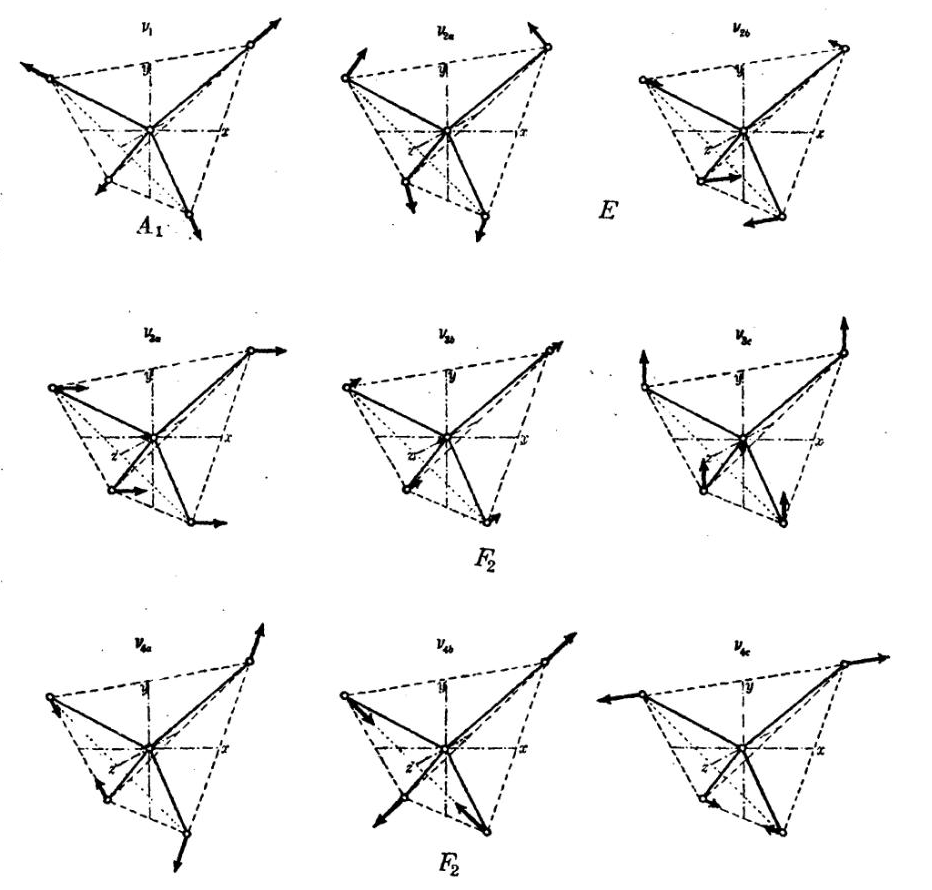
\includegraphics[width=\textwidth]{figures/tetraeder.png}
          \caption[Mögliche Schwingungen eines tetraedischen $\mathrm{XY_4}$-Moleküls.]{Mögliche Schwingungen eines tetraedischen $\mathrm{XY_4}$-Moleküls. Offenbar sind die Schwingungen der zweiten und dritten Zeile energetisch entartet (vgl. \cref{subsec:tetrachlor}). \cite{herzberg}}
          \label{fig:tetraeder-schwingungen}
        \end{figure}

        Die verbleibenden beiden Schwingungen können an dieser Stelle noch nicht zugeordnet werden.


      \subsection{Chloroform und Deuterochloroform}

        \Cref{fig:chcl3-cdcl3} zeigt die Spektren von Chloroform ($\mathrm{CHCl_3}$) und Deuterochloroform ($\mathrm{CDCl_3}$). Im Vergleich der jeweiligen Spektren mit Polarisationsfilter in Nullstellung und um $\ang{90}$ gedrehter Stellung fällt sofort auf, dass drei der sechs für beide Moleküle erscheinenden Maxima zu symmetrischen Schwingungen gehören. 

        \begin{figure}[p]
          \subfloat{
            \tikzsetnextfilename{CHCl3}
            \begin{tikzpicture}
              \begin{axis}[
                /tikz/line join=bevel,
                width=0.8*\textwidth,
                height=0.5*\textwidth,
                grid,
                legend style={at={(1,1)}, legend columns=1, anchor=north east},
                every axis plot,
                xmin = 0, xmax = 3100,
                %ymin = \Pmin, ymax = \Pmax,
                xlabel = {Raman-Verschiebung $\Delta \nu$ in $\si{\per\centi\meter}$},
                ylabel = {Zählrate $n$},
                /pgf/number format/use comma,
                /pgf/number format/1000 sep={},
                ]
                % Add plots
                \addplot[color=red,  line width = 1pt] table [x=raman,y=n]{data/CHCl3_pol0.txt};
                \addlegendentry{$\theta_\mathrm{pol}=\ang{0}$}
                \addplot[color=blue,  line width = 1pt] table [x=raman,y=n]{data/CHCl3_pol1.txt};
                \addlegendentry{$\theta_\mathrm{pol}=\ang{90}$}
              \end{axis}
            \end{tikzpicture}
            \label{fig:chcl3}}  \\
          \subfloat{
            \tikzsetnextfilename{CDCl3}
            \begin{tikzpicture}
              \begin{axis}[
                /tikz/line join=bevel,
                width=0.8*\textwidth,
                height=0.5*\textwidth,
                grid,
                legend style={at={(1,1)}, legend columns=1, anchor=north east},
                every axis plot,
                xmin = 0, xmax = 3100,
                %ymin = \Pmin, ymax = \Pmax,
                xlabel = {Raman-Verschiebung $\Delta \nu$ in $\si{\per\centi\meter}$},
                ylabel = {Zählrate $n$},
                /pgf/number format/use comma,
                /pgf/number format/1000 sep={},
                ]
                % Add plots
                \addplot[color=red,  line width = 1pt] table [x=raman,y=n]{data/CDCl3_pol0.txt};
                \addlegendentry{$\theta_\mathrm{pol}=\ang{0}$}
                \addplot[color=blue,  line width = 1pt] table [x=raman,y=n]{data/CDCl3_pol1.txt};
                \addlegendentry{$\theta_\mathrm{pol}=\ang{90}$}
              \end{axis}
            \end{tikzpicture}
            \label{fig:cdcl3}}
          \caption{Spektren von $\mathrm{CHCl_3}$ \protect\subref{fig:chcl3} und $\mathrm{CDCl_3}$ \protect\subref{fig:cdcl3} mit Polarisationsfilter in Nullstellung und um $\ang{90}$ gedrehtem Filter.}
          \label{fig:chcl3-cdcl3}
        \end{figure}




\end{document}
